\hypertarget{manger-au-liban}{%
\section{Manger au Liban}\label{manger-au-liban}}

\emph{Mercredi 23 mai 2018}

Comme je l'ai déjà écrit dans le premier billet sur le Liban, nous avons
été accueilli de manière extrêmement généreuse par la famille d'Elida.
Tout le monde s'occupe de nous, nous propose des excursions, demande
comment je trouve le Liban et... nous invite à manger. Cela se traduit
principalement par deux choses : la commande d'un nombre extraordinaire
de plats, bien au-delà du raisonnable, et le fait qu'on ressort de table
après plusieures heures en n'ayant plus du tout faim :D

\begin{figure}
\centering
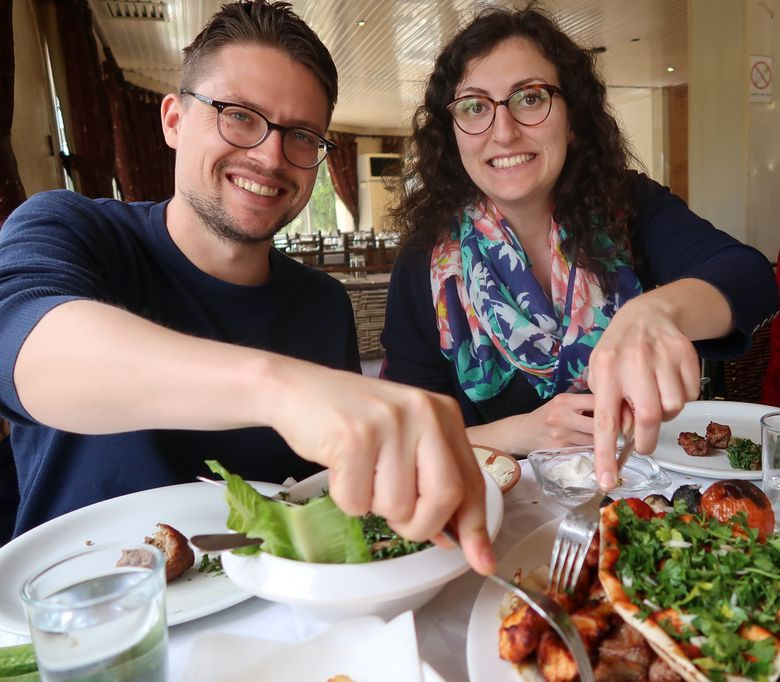
\includegraphics{images/20180523_manger.JPG}
\caption{Exemple de festin sur fond de gastronomes heureux.}
\end{figure}

Le déroulement d'un repas peut être décrit par la séquence suivante :

\begin{itemize}
\tightlist
\item
  on amène des petites choses à grignoter à la table (par exemple :
  olives, amandes vertes qu'on mange en entier, petits pois,
  cacahouètes)
\item
  le serveur demande "Fattoush ou Tabbouleh ?" et prend la commande des
  mezzés et des plats
\item
  le serveur sert le Fattoush / Tabbouleh, puis les mezzés arrivent et
  on en mange avec du pain libanais qu'on déchire pour former des petits
  récipients pour aller "pêcher" du Hommous et du Labneh
\item
  on n'a plus faim car tout est très bon et on a eu envie de tout goûter
\item
  les grillades (kefta, taouk de poulet, brochettes de boeuf) arrivent,
  on est surpris car on ne s'y attendait plus, et on en mange même si on
  a plus faim
\item
  on n'a vraiment plus faim
\item
  on passe au dessert (fruits frais, gâteau d'anniversaire ou de baptême
  s'il y a lieu, gâteaux pleins de sirop de sucre)
\end{itemize}

Optionnellement, on peut bien entendu commander un narguilé (qu'on
appelle d'ailleurs arguilé ici) que l'on "déguste" au fil du repas.

On peut noter que par rapport au repas français traditionnel, le repas
libanais ne s'accompagne pas forcément d'un café à la fin (je me suis
rendu compte qu'on sert le café "à la turque" à n'importe quelle heure
de la journée, et qu'il est généralement moins fort que le café que l'on
a coutume de boire en France).

Concernant les boissons alcoolisées, l'Arak occupe une place de premier
choix sur la table libanaise. Qu'il soit fait maison ou pas, on en
rencontre bien plus souvent que le vin de nos contrées.

Vous l'aurez compris, on mange bien au Liban.

Malheureusement, ceci m'amène au revers de la médaille : au restaurant,
ce qui est commandé mais n'a pas pu être mangé par les convives finit...
à la poubelle ! La culture de l'hospitalité prescrit un festin, mais ne
prévoit pas (encore ?) de garder les restes et de les ramener à la
maison.

Allez, on vous laisse saliver avec nos photos de repas libanais !

\emph{Florian}

\hypertarget{commentaires}{%
\subsection{Commentaires}\label{commentaires}}

\begin{itemize}
\item
  Thibaud, \emph{2018-05-24 16h06}

  C'est le genre d'article qui me donne envie de partir :D\\
  Merci pour les légendes ! N'oubliez pas quand même qu'on a des fraises
  et des pommes chez nous. On dirait la documentation d'Alex sur un
  constructeur : "// Constructor."\\
  (Ceci est un test pour voir si l'intéressé parcourt votre blog :p)
\item
  Florian LB, \emph{2018-05-26 09h55}

  Haha c'est le genre de réaction qu'on espérait provoquer ;)\\
  On oublie pas qu'on a des pommes et des fraises en France, c'est juste
  qu'on n'arrive pas à ne pas être exhaustifs dans notre collecte de
  photos \^{}\^{}\\
  Pour l'instant je n'ai pas encore eu de commentaire de la part d'Alex,
  mais j'imagine que ça ne va pas tarder...
\item
  kje, \emph{2018-05-28 21h09}

  Du coup, une préférence entre le taboulé de la cantine 3 et celui que
  tu manges au Liban ?
\item
  Florian LB, \emph{2018-06-01 08h51}

  Rien à voir ! Mais j'imagine que tu connaissais déjà la réponse à
  cette question... Pour ceux qui n'ont pas été confronté à cette
  expérience : "taboulé" est un terme qui recouvre un grand nombre de
  plats très différents les uns des autres. Il faudrait sans doute
  exiger un adjectif obligatoire quand on l'utilise pour éviter les
  ambiguïtés.
\item
  pythux, \emph{2018-05-31 10h15}

  Excellent Flo ! Ça fait saliver tout ça :) Ça me rappel le classique
  "dîner chez les potes indiens" : "Allez on passe à table ?"; "Quoi ?
  Je croyais qu'on avait fini là", et "hé non, c'était l'apéritif !"...
  Je me fait avoir à chaque fois.
\item
  Florian LB, \emph{2018-06-01 08h53}

  Je ne savais pas que la gastronomie indienne avait ce point commun
  avec la libanaise. C'est ça de faire des plats apéritifs trop bons...
\item
  Timothée Nicolas, \emph{2018-06-03 20h56}

  Omg ça a l'air tellement bon ! C'était bon la barbaque crue ? J'avais
  toujours eu du mal à imaginer quand Farah disait qu'elle bouffait du
  foie d'agneau cru au petit déj. T'as goûté ? C'est bon ?
\item
  Florian LB, \emph{2018-06-04 06h56}

  J'ai seulement goûté et il faut dire que cela a un goût assez fort.
  Donc je n'irais pas jusqu'à dire que j'ai apprécié. Heureusement que
  ce n'était pas au petit déjeuner mais au déjeuner chez nous...
\end{itemize}

